\documentclass[a4paper]{book}

% Packages
\usepackage{graphicx}
\usepackage{geometry}
\usepackage{hyperref}
\usepackage[utf8]{vietnam}
\usepackage{amsmath}
\usepackage{amssymb}
\usepackage{float}
\usepackage{algorithm}
\usepackage{algorithmic}
\usepackage{listings}
\usepackage{url}

% Geometry setup
\geometry{left=2cm,right=2cm,top=2cm,bottom=2cm}

% Titlepage information
\newcommand{\reporttitle}{Hệ thống điểm danh nhân viên sử dụng nhận diện khuôn mặt}
\newcommand{\reportauthors}{%
    Nguyễn Hữu Duy
}
\newcommand{\courseinfo}{Mã học phần: MAT3508\\ Học kỳ 1, Năm học 2025-2026}
\newcommand{\universitylogo}{HUS.png} % Đặt file logo vào cùng thư mục

\newcommand{\doi}[1]{\href{https://doi.org/#1}{\texttt{#1}}} % DOI link command


% Loại bỏ trang trắng thừa đầu chương (book class)
\let\cleardoublepage\clearpage
\begin{document}

% Trang bìa
\begin{titlepage}
    \centering
    \vspace*{-1cm}
    {\LARGE\MakeUppercase{Đại học Quốc gia Hà Nội}\par}
    {\LARGE\MakeUppercase{Trường Đại học Khoa học Tự nhiên}\par}
    \vfill
    \includegraphics[width=0.3\textwidth]{\universitylogo}\par\vfill
    {\Huge \bfseries \reporttitle \par}
    \vspace{1cm}
    {\Large \reportauthors \par}
    \vspace{1cm}
    {\large \courseinfo \par}
    \vfill
\end{titlepage}
% Trang thông tin dự án
\clearpage
\thispagestyle{empty}
\begin{center}
    {\LARGE \textbf{Thông tin Dự án}}\\[1.5em]
    \parbox{0.85\textwidth}{
    }
    \\[2em]
    \begin{tabular}{rl}
        \textbf{Học phần:} & MAT3508 -- Nhập môn Trí tuệ Nhân tạo \\
        \textbf{Học kỳ:} & Học kỳ 1, Năm học 2025-2026 \\
        \textbf{Trường:} & VNU-HUS (Đại học Quốc gia Hà Nội -- Trường Đại học Khoa học Tự nhiên) \\
        \textbf{Tên dự án:} & {[Tên dự án của bạn]} \\
        \textbf{Ngày nộp:} & {[Ngày nộp]} (ví dụ: 30/06/2025) \\
        \textbf{Báo cáo PDF:} & \href{https://github.com/23001853-wq/Employee-Attendance-System-Using-Camera/blob/main/report.pdf}{Liên kết tới báo cáo PDF trong kho GitHub} \\
        \textbf{Slide thuyết trình:} & \href{https://github.com/23001853-wq/Employee-Attendance-System-Using-Camera/blob/main/slides.pdf}{Liên kết tới slide thuyết trình trong kho GitHub} \\
        \textbf{Kho GitHub:} & \url{https://github.com/23001853-wq/Employee-Attendance-System-Using-Camera.git}
    \end{tabular}
    \\[2em]
    {\Large \textbf{Thành viên nhóm}}\\[1em]
    \begin{tabular}{|l|l|l|l|}
        \hline
        \textbf{Họ tên} & \textbf{Mã sinh viên} & \textbf{Tên GitHub}  \\
        \hline
        (Nguyễn Hữu Duy) & (23001853) & (23001853-wq)  \\
        \hline
     
    \end{tabular}
\end{center}
\tableofcontents
\clearpage
% Chương 1: Giới thiệu
\chapter{Giới thiệu}

\section{Tóm tắt}
Hệ thống điểm danh tự động dựa trên nhận diện khuôn mặt sử dụng học sâu (Deep Learning) được phát triển nhằm thay thế phương pháp điểm danh thủ công, nâng cao độ chính xác và tự động hóa. Dữ liệu khuôn mặt được thu thập qua webcam, tiền xử lý và lưu trữ, trước khi trích xuất đặc trưng bằng mạng MobileNetV2. Các vector đặc trưng 1280 chiều sau đó được **chuẩn hóa L2** để đảm bảo độ ổn định và độ chính xác khi đưa vào các thuật toán phân loại.

Trước khi trích xuất vector, hệ thống sử dụng thuật toán Haar Cascade của OpenCV để phát hiện và cắt vùng khuôn mặt, giúp xử lý tốt các điều kiện ánh sáng khác nhau và đảm bảo vector đầu vào chỉ chứa khuôn mặt. Các thuật toán phân loại được áp dụng gồm: SVM, KNN, Random Forest (học có giám sát) và Cosine Similarity, L2 Distance (học không giám sát), từ đó so sánh để lựa chọn giải pháp tối ưu.

Kết quả thực nghiệm cho thấy SVM (RBF Kernel) kết hợp chuẩn hóa L2 đạt độ chính xác cao nhất, nhận diện ổn định, thời gian xử lý nhanh và phù hợp triển khai thực tế. Hệ thống còn có giao diện \textbf{Streamlit} thân thiện, tích hợp cơ sở dữ liệu \textbf{SQL Server} để quản lý thông tin nhân viên và lịch sử điểm danh, đồng thời hỗ trợ tăng cường dữ liệu tự động nhằm cải thiện hiệu quả nhận diện.

\section{Bài toán đặt ra}
Điểm danh truyền thống bằng giấy tờ hoặc thẻ từ dễ gian lận, tốn thời gian và không phù hợp với quá trình chuyển đổi số. Bài toán đặt ra là xây dựng hệ thống điểm danh tự động, nhận diện chính xác khuôn mặt nhân viên trong điều kiện thực tế, đảm bảo an ninh, dễ sử dụng và có khả năng mở rộng.

\section{Thách thức}
Hệ thống cần giải quyết các thách thức sau:
\begin{enumerate}
    \item \textbf{Đảm bảo độ chính xác cao với dữ liệu nhỏ:} Số lượng ảnh mỗi nhân viên ít, cần thuật toán học sâu nhẹ kết hợp SVM/KNN/RF để đạt hiệu quả mà không quá khớp.
    \item \textbf{Xử lý đa dạng khuôn mặt và điều kiện ánh sáng:} Haar Cascade phát hiện khuôn mặt trên ảnh xám để tăng độ chính xác, sau đó cắt và lấy lại vùng mặt từ ảnh gốc màu trước khi trích xuất vector đặc trưng.
    \item \textbf{Chuẩn hóa L2 và tối ưu tốc độ nhận diện:} Vector 1280 chiều từ MobileNetV2 được chuẩn hóa L2 và đưa vào SVM cho phép nhận diện nhanh, đủ cho ứng dụng real-time.
    \item \textbf{So sánh nhiều thuật toán:} Học có giám sát và không giám sát để chọn mô hình tối ưu về độ chính xác, tốc độ và khả năng mở rộng.
    \item \textbf{Quản lý check-in/check-out và cơ sở dữ liệu:} Sau khi nhận diện, hệ thống ghi nhận thời gian vào/ra nhân viên vào SQL Server, hỗ trợ tra cứu lịch sử và báo cáo.
    \item \textbf{Khả năng mở rộng:} Thiết kế để mở rộng khi số lượng nhân viên tăng hoặc dữ liệu lớn hơn, dễ tích hợp các thuật toán Deep Learning nâng cao như ArcFace.
\end{enumerate}


\chapter{Phương pháp \& Triển khai}

\section{Phương pháp}
Pipeline nhận diện khuôn mặt được xây dựng dựa trên quy trình xử lý ảnh tiêu chuẩn, bao gồm ba giai đoạn chính: Thu thập dữ liệu đầu vào, Phát hiện khuôn mặt (Face Detection) và Tiền xử lý dữ liệu (Preprocessing).

\subsection{Thu thập dữ liệu (Data Collection)}
Dữ liệu đầu vào đóng vai trò quyết định đến độ chính xác của mô hình. Hệ thống hỗ trợ hai phương thức thu thập dữ liệu:

\begin{enumerate}
    \item \textbf{Thu thập trực tiếp qua Webcam:}
    \begin{itemize}
        \item Hệ thống kích hoạt camera và tự động chụp liên tục khuôn mặt người dùng trong thời gian thực.
        \item Mỗi nhân viên sẽ được chụp khoảng 50 mẫu ảnh ở các góc độ và điều kiện ánh sáng khác nhau.
        \item Dữ liệu được gán nhãn với ID định danh (khóa chính) để phục vụ quá trình huấn luyện.
    \end{itemize}
    
    \begin{figure}[h!]
        \centering
        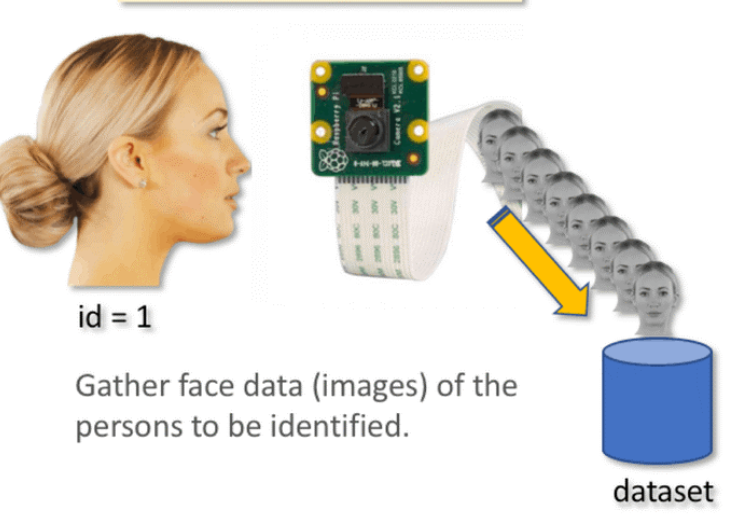
\includegraphics[width=0.5\textwidth]{annh1.png}
        \caption{Giao diện thu thập dữ liệu trực tiếp từ Webcam - nhân viên nhìn thẳng vào camera để chụp nhiều góc độ khác nhau.}
        \label{fig:webcam-capture}
    \end{figure}

    \item \textbf{Thu thập từ nguồn ảnh có sẵn (Static Images):}
    \begin{itemize}
        \item Đối với các nhân viên không thể có mặt trực tiếp hoặc dữ liệu người nổi tiếng, hệ thống cho phép nhập dữ liệu từ kho ảnh tĩnh.
        \item \textbf{Quy trình:} Tập hợp ảnh chân dung nhân viên (khuyến khích chọn ảnh đa dạng bối cảnh). Hệ thống sẽ quét thư mục, sử dụng thuật toán Haar Cascade để cắt lấy khuôn mặt và lưu vào tập dữ liệu huấn luyện.
    \end{itemize}
    
    \begin{figure}[h!]
        \centering
        
\includegraphics[width=0.5\textwidth]{musk.jpg}
        \caption{Ví dụ thu thập dữ liệu từ ảnh tĩnh (Elon Musk) - ảnh chân dung.}
        \label{fig:static-image-capture}
    \end{figure}
\end{enumerate}

\subsection{Phát hiện và cắt khuôn mặt (Face Detection)}
Để xác định vị trí khuôn mặt trong ảnh và loại bỏ nền, hệ thống sử dụng thuật toán \textbf{Viola-Jones (Haar Cascade)}. Đây là phương pháp máy học có tốc độ xử lý cực nhanh và độ chính xác cao, hoạt động dựa trên các thành phần cốt lõi sau:

\subsubsection{Đặc trưng Haar-like (Haar-like Features)}
Thuật toán Viola-Jones sử dụng các đặc trưng Haar-like thay vì xử lý trực tiếp giá trị pixel. Những đặc trưng này được thiết kế để nắm bắt các đặc điểm cấu trúc quan trọng của khuôn mặt:

\begin{itemize}
    \item \textbf{Đặc trưng 2-rectangle:} Phát hiện các cạnh và biên giới sáng-tối (ví dụ: hốc mắt tối hơn má).
    \item \textbf{Đặc trưng 3-rectangle:} Nhận diện các đường kẻ và vạch (ví dụ: sống mũi, miệng).
    \item \textbf{Đặc trưng 4-rectangle:} Phát hiện các mẫu chéo và đối xứng (ví dụ: đặc điểm chéo của mắt).
\end{itemize}

Công thức tính giá trị đặc trưng Haar:
\[
\text{Feature\_Value} = \sum_{\text{White}} I(x,y) - \sum_{\text{Black}} I(x,y)
\]

\begin{figure}[h!]
\centering
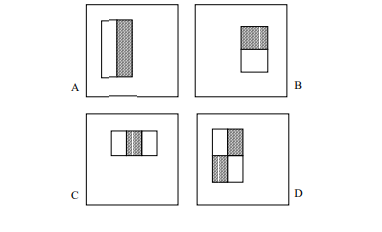
\includegraphics[width=0.6\textwidth]{anhmh1.png}
\caption{\textbf{Các loại đặc trưng Haar-like cơ bản:} (A) 2-rectangle dọc - phát hiện cạnh dọc, (B) 2-rectangle ngang - phát hiện cạnh ngang, (C) 3-rectangle - phát hiện đường kẻ và mũi, (D) 4-rectangle - phát hiện vùng mắt và các đặc trưng đối xứng. Vùng trắng có trọng số +1, vùng đen có trọng số -1.}
\label{fig:haar-features}
\end{figure}

\subsubsection{Ảnh tích hợp (Integral Image)}
Để tăng tốc độ tính toán đặc trưng Haar từ $O(n^2)$ xuống $O(1)$, thuật toán sử dụng \textit{Ảnh tích hợp}. Ảnh tích hợp tại điểm $(x, y)$ lưu trữ tổng tích lũy của tất cả pixel từ góc trên-trái $(0,0)$ đến điểm hiện tại:

\[
ii(x,y) = \sum_{x' \leq x, y' \leq y} i(x',y')
\]

\textbf{Công thức tính nhanh tổng vùng chữ nhật:}
Với 4 điểm góc A, B, C, D của hình chữ nhật, tổng pixel trong vùng được tính chỉ bằng 4 phép truy cập mảng:
\[
\text{Sum}(D) = 4 + 1 - (2 + 3)
\]
*(Ký hiệu theo sơ đồ minh họa dưới đây)*

\begin{figure}[h!]
\centering
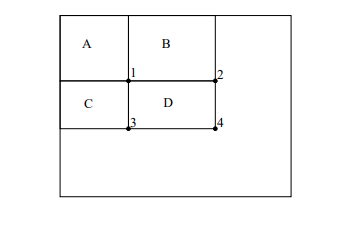
\includegraphics[width=0.5\textwidth]{anhmh2.png}
\caption{\textbf{Minh họa Integral Image:} (Trái) Giá trị ảnh tích hợp tại điểm 1, 2, 3, 4. (Phải) Tổng pixel của vùng D được tính nhanh bằng công thức: $Sum(D) = ii(4) + ii(1) - ii(2) - ii(3)$.}
\label{fig:integral-image}
\end{figure}

\subsubsection{Cấu trúc Cascade (Attentional Cascade)}
Để đạt hiệu quả thời gian thực (real-time), thuật toán sử dụng cấu trúc \textit{cascade of classifiers} - một chuỗi các bộ phân loại từ đơn giản đến phức tạp.
Cơ chế này hoạt động như một "cây quyết định suy biến" (degenerate decision tree):
\begin{itemize}
    \item Các stage đầu loại bỏ nhanh phần lớn (khoảng 50\%) các vùng "chắc chắn không phải mặt" với chi phí tính toán rất thấp.
    \item Chỉ những vùng vượt qua được các stage đầu mới được xử lý bởi các stage phức tạp hơn phía sau.
\end{itemize}

\begin{figure}[h!]
\centering
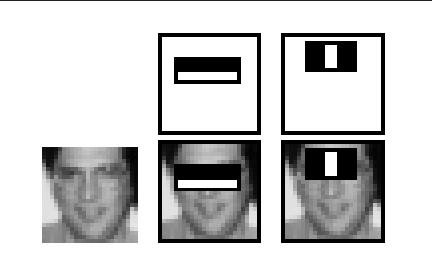
\includegraphics[width=0.6\textwidth]{anhmh3.png}
\caption{\textbf{Cấu trúc Cascade Classifier:} Luồng xử lý đi qua các stage nối tiếp. Nếu vùng ảnh bị từ chối (F) ở bất kỳ stage nào, nó sẽ bị loại bỏ ngay lập tức. Chỉ vùng được chấp nhận (T) qua tất cả các stage mới được kết luận là khuôn mặt.}
\label{fig:cascade-structure}
\end{figure}

\subsubsection{Dữ liệu huấn luyện gốc (Training Dataset)}
Hiệu năng của thuật toán Haar Cascade phụ thuộc vào tập dữ liệu mà nó đã được huấn luyện (trong thư viện OpenCV). Theo bài báo gốc của Viola và Jones, tập dữ liệu này bao gồm:
\begin{itemize}
    \item \textbf{Positive samples:} 4,916 ảnh khuôn mặt được gán nhãn thủ công, chuẩn hóa về kích thước 24×24 pixels.
    \item \textbf{Negative samples:} 9,544 ảnh không chứa khuôn mặt (phong cảnh, vật thể) để tạo ra các mẫu âm tính.
\end{itemize}

\begin{figure}[h!]
\centering
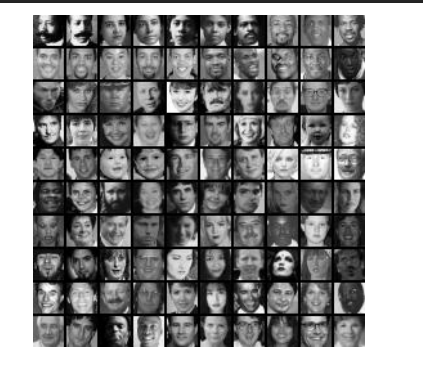
\includegraphics[width=0.65\textwidth]{anhmh5.png} % Đảm bảo đây là ảnh Figure 5 từ PDF
\caption{\textbf{Mẫu dữ liệu huấn luyện (MIT-CMU database):} Các khuôn mặt được sử dụng để huấn luyện là ảnh xám, nhìn thẳng (frontal) và đứng (upright).}
\label{fig:training-samples}
\end{figure}

\textbf{Tác động của dữ liệu huấn luyện đến hệ thống thực tế:}
\begin{itemize}
    \item \textbf{Yêu cầu về tư thế:} Do được huấn luyện trên các ảnh \textit{frontal upright} (như hình trên), thuật toán hoạt động tốt nhất khi người dùng nhìn thẳng. Hệ thống chỉ chấp nhận độ nghiêng đầu giới hạn trong khoảng $\pm 15^\circ$.
    \item \textbf{Cơ sở tiền xử lý:} Việc mô hình gốc học trên ảnh xám (grayscale) và ảnh cắt sát mặt là cơ sở để nhóm thực hiện các bước tiền xử lý tương tự (chuyển xám, crop) nhằm đảm bảo dữ liệu đầu vào tương thích nhất với thuật toán.
\end{itemize}

\subsection{Tiền xử lý và Tăng cường dữ liệu (Preprocessing \& Augmentation)}
Sau khi khuôn mặt được phát hiện, dữ liệu được chuẩn hóa trước khi đưa vào mô hình nhận diện:

\begin{enumerate}
    \item \textbf{Chuyển đổi thang đo xám (Grayscale conversion):} \\
Ảnh đầu vào được chuyển sang ảnh xám bằng hàm \texttt{cv2.cvtColor}. 
Bước này giúp giảm nhiễu màu và giảm khối lượng tính toán, đồng thời phù hợp với yêu cầu đầu vào của thuật toán phát hiện khuôn mặt Haar Cascade nhằm tìm vị trí mặt một cách nhanh và chính xác hơn.

\item \textbf{Chuẩn hóa kích thước (Resizing):} \\
Sau khi khuôn mặt được cắt ra từ ảnh gốc, ảnh được đưa về kích thước chuẩn \textbf{224×224 pixel}. 
Điều này đảm bảo tính nhất quán cho vector đặc trưng đầu vào của mô hình trích xuất đặc trưng và nhận diện.

\item \textbf{Tăng cường dữ liệu (Data Augmentation):} \\
Để mô hình hoạt động ổn định trong nhiều điều kiện thực tế, tập dữ liệu được mở rộng bằng các phép biến đổi ngẫu nhiên, gồm:
\begin{itemize}
    \item \textbf{Lật ảnh (Horizontal flipping):} Tạo biến thể khuôn mặt trái/phải.
    \item \textbf{Xoay ảnh (Rotation ±20°):} Mô phỏng trường hợp người dùng hơi nghiêng đầu.
    \item \textbf{Tịnh tiến (Width/Height shifting):} Dịch chuyển khuôn mặt để tăng đa dạng vị trí.
    \item \textbf{Thu phóng (Zoom):} Phóng to hoặc thu nhỏ nhằm mô phỏng thay đổi khoảng cách camera.
    \item \textbf{Biến dạng cắt xiên (Shear):} Tạo biến đổi hình dạng nhẹ để tăng khả năng khái quát.
    \item \textbf{Điều chỉnh độ sáng (Brightness adjustment):} Giúp mô hình thích nghi với điều kiện ánh sáng khác nhau.
\end{itemize}

\begin{figure}[h!]
\centering
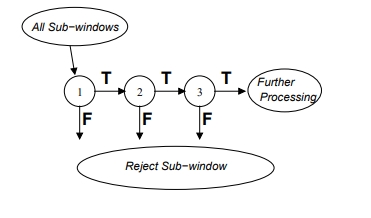
\includegraphics[width=0.9\textwidth]{anhmh4.png}
\caption{\textbf{Ví dụ các phép biến đổi trong Data Augmentation} được áp dụng lên ảnh khuôn mặt.}
\label{fig:augmentation-examples}
\end{figure}
\end{enumerate}

\subsection{Trích xuất Đặc trưng với MobileNetV2}

\subsubsection{Lý do chọn MobileNetV2}
MobileNetV2 là kiến trúc CNN (Convolutional Neural Network) được Google phát triển năm 2018, đặc biệt tối ưu cho các thiết bị có tài nguyên hạn chế. Đây là lựa chọn phù hợp cho dự án vì:

\begin{itemize}
    \item \textbf{Hiệu suất cao với tài nguyên thấp:} MobileNetV2 sử dụng \textit{depthwise separable convolution} và \textit{inverted residual blocks}, giúp giảm số lượng phép toán so với các CNN truyền thống (VGG, ResNet) nhưng vẫn duy trì độ chính xác cao.
    
    \item \textbf{Pretrained trên ImageNet:} Mô hình đã được Google huấn luyện sẵn trên dataset ImageNet (hơn 14 triệu ảnh, 1000 lớp), do đó có khả năng trích xuất đặc trưng hình ảnh tổng quát rất tốt mà không cần huấn luyện lại từ đầu.
    
    \item \textbf{Transfer Learning:} Trong dự án này, nhóm \textbf{không huấn luyện lại} MobileNetV2, mà chỉ sử dụng nó như một \textit{feature extractor} (trích xuất đặc trưng). Đây là cách tiếp cận hiệu quả khi không có đủ dữ liệu và tài nguyên GPU để huấn luyện một CNN từ đầu.
    
    \item \textbf{Vector đặc trưng 1280 chiều:} Output của lớp cuối cùng (trước lớp phân loại) cho ra vector 1280 chiều, đủ mạnh để phân biệt các khuôn mặt khác nhau.
\end{itemize}

\subsubsection{Kiến trúc CNN và MobileNetV2}
\textbf{Convolutional Neural Network (CNN)} là loại mạng nơ-ron chuyên xử lý dữ liệu dạng lưới (như ảnh), bao gồm các lớp chính:
\begin{itemize}
    \item \textbf{Convolutional Layer:} Trích xuất các đặc trưng cục bộ (cạnh, góc, texture) bằng các kernel/filter.
    \item \textbf{Pooling Layer:} Giảm kích thước không gian, giữ lại thông tin quan trọng.
    \item \textbf{Fully Connected Layer:} Kết hợp các đặc trưng để đưa ra dự đoán cuối cùng.
\end{itemize}

\textbf{MobileNetV2} cải tiến bằng \textit{Inverted Residual Block}:
\[
\text{Input} \xrightarrow{\text{Expand (1×1 conv)}} \text{High-dim} \xrightarrow{\text{Depthwise (3×3)}} \text{Spatial} \xrightarrow{\text{Project (1×1)}} \text{Low-dim Output}
\]

Cấu trúc này giúp giảm đáng kể số lượng tham số so với CNN truyền thống, phù hợp cho triển khai thực tế.

\subsubsection{Quy trình Trích xuất Đặc trưng}
\begin{enumerate}
    \item \textbf{Load mô hình pretrained:} 
    \begin{itemize}
        \item Sử dụng \texttt{tf.keras.applications.MobileNetV2} với trọng số đã huấn luyện trên ImageNet.
        \item Loại bỏ lớp phân loại cuối cùng (\texttt{include\_top=False}), chỉ giữ lại phần trích xuất đặc trưng.
    \end{itemize}
    
    \item \textbf{Trích xuất vector 1280 chiều:} 
    \begin{itemize}
        \item Mỗi ảnh khuôn mặt $224 \times 224 \times 3$ được đưa qua MobileNetV2.
        \item Output là tensor $7 \times 7 \times 1280$, sau đó được \textit{Global Average Pooling} thành vector $1280$ chiều.
    \end{itemize}
    
    \item \textbf{Chuẩn hóa L2 (L2 Normalization):} 
    
    \textbf{Vì sao cần chuẩn hóa L2?}
    
    Vector đặc trưng từ MobileNetV2 có giá trị không đồng nhất - một số chiều có giá trị rất lớn, một số rất nhỏ. Nếu sử dụng trực tiếp, các thuật toán phân loại sẽ gặp vấn đề:
    
    \begin{itemize}
        \item \textbf{Độ lớn vector không đồng nhất:} Ảnh sáng hơn có thể tạo ra vector với norm lớn hơn, dẫn đến khoảng cách Euclid bị ảnh hưởng bởi độ sáng thay vì nội dung khuôn mặt.
        
        \item \textbf{Scale khác nhau:} SVM và KNN hoạt động dựa trên khoảng cách - nếu các chiều có scale khác nhau, các chiều có giá trị lớn sẽ "chi phối" kết quả.
        
        \item \textbf{Cosine Similarity yêu cầu:} Thuật toán Cosine chỉ quan tâm đến \textit{hướng} của vector, không quan tâm độ dài. Chuẩn hóa L2 giúp tất cả vector có độ dài = 1, biến khoảng cách Euclid tương đương với Cosine distance.
    \end{itemize}
    
    \textbf{Công thức và cách hoạt động:}
    \[
    v_{\text{norm}} = \frac{v}{\|v\|_2} = \frac{v}{\sqrt{\sum_{i=1}^{1280} v_i^2}}
    \]
    
    \textbf{Ví dụ minh họa:}
    
    Giả sử vector gốc: $v = [3, 4, 0, 0, \ldots, 0]$ (1280 chiều, phần lớn = 0)
    
    \begin{enumerate}
        \item Tính norm L2: $\|v\|_2 = \sqrt{3^2 + 4^2} = \sqrt{9 + 16} = 5$
        \item Chia từng phần tử cho norm: $v_{\text{norm}} = \left[\frac{3}{5}, \frac{4}{5}, 0, \ldots, 0\right] = [0.6, 0.8, 0, \ldots, 0]$
        \item Kiểm tra: $\|v_{\text{norm}}\|_2 = \sqrt{0.6^2 + 0.8^2} = \sqrt{0.36 + 0.64} = 1$
    \end{enumerate}
    
    \textbf{Lợi ích sau khi chuẩn hóa:}
    
    \begin{itemize}
        \item \textbf{Tất cả vector có cùng độ dài = 1:} Loại bỏ ảnh hưởng của độ sáng, chỉ so sánh "hướng" (nội dung khuôn mặt).
        
        \item \textbf{Khoảng cách có ý nghĩa hơn:} Với hai vector chuẩn hóa $a$ và $b$:
        \[
        \|a - b\|_2^2 = 2(1 - a \cdot b) = 2(1 - \cos(\theta))
        \]
        Tức là khoảng cách Euclid tỷ lệ thuận với góc giữa hai vector.
        
        \item \textbf{Hội tụ nhanh hơn:} SVM và các thuật toán gradient-based hoạt động ổn định hơn khi dữ liệu có cùng scale.
    \end{itemize}
    
    \item \textbf{Gán nhãn:} Mỗi vector đặc trưng đã chuẩn hóa được gán nhãn theo ID nhân viên (nhanvien\_1, nhanvien\_2, ...).
\end{enumerate}

\subsection{So sánh Thuật toán Phân loại}
Sau khi có vector đặc trưng, bước tiếp theo là chọn thuật toán phân loại phù hợp. Nhóm đã so sánh 5 thuật toán khác nhau:

\subsubsection{1. Support Vector Machine (SVM) với RBF Kernel}
\textbf{Ý tưởng:} SVM tìm siêu phẳng (hyperplane) tối ưu để phân tách các lớp dữ liệu với margin lớn nhất.

\textbf{Công thức:}
\[
f(x) = \text{sign}\left(\sum_{i=1}^{N} \alpha_i y_i K(x_i, x) + b\right)
\]
Trong đó, \textit{RBF (Radial Basis Function) Kernel} được định nghĩa:
\[
K(x_i, x_j) = \exp\left(-\gamma \|x_i - x_j\|^2\right)
\]

\subsubsection{2. K-Nearest Neighbors (KNN)}
\textbf{Ý tưởng:} Phân loại dựa trên "đa số bầu chọn" từ $k$ láng giềng gần nhất.

\textbf{Công thức:}
\[
\text{label}(x) = \text{mode}\left(\{ \text{label}(x_i) \mid x_i \in k \text{ nearest neighbors of } x \}\right)
\]

\subsubsection{3. Random Forest}
\textbf{Ý tưởng:} Kết hợp nhiều cây quyết định (decision trees), mỗi cây được huấn luyện trên tập con ngẫu nhiên của dữ liệu.

\textbf{Công thức dự đoán:}
\[
\hat{y} = \text{mode}\left(\{ h_1(x), h_2(x), \ldots, h_T(x) \}\right)
\]
Trong đó $h_t(x)$ là dự đoán của cây thứ $t$, và $T$ là tổng số cây.

\subsubsection{4. Cosine Similarity (Phương pháp Nearest Class Centroid)}

\textbf{Ý tưởng:} Thay vì so sánh với toàn bộ dữ liệu huấn luyện như KNN, phương pháp này tính toán một \textbf{vector đại diện} (template/prototype) cho mỗi nhân viên bằng cách lấy trung bình cộng của tất cả các vector đặc trưng thuộc về nhân viên đó:

\[
\text{template}_c = \frac{1}{N_c} \sum_{i: y_i = c} x_i
\]

Trong đó $N_c$ là số lượng ảnh của nhân viên $c$. Vector trung bình này đóng vai trò là "tâm" (centroid) của cụm dữ liệu, giúp loại bỏ nhiễu và các đặc điểm ngoại lai (outliers) của từng ảnh riêng lẻ, tạo ra một chân dung đặc trưng "ổn định" nhất của nhân viên.

Khi kiểm thử, hệ thống so sánh ảnh đầu vào với các vector đại diện này bằng độ đo Cosine Similarity:

\[
\text{similarity}(x, \text{template}_c) = \cos(\theta) = \frac{x \cdot \text{template}_c}{\|x\|_2 \|\text{template}_c\|_2}
\]

Nhãn dự đoán là lớp có độ tương đồng cao nhất:
\[
\hat{y} = \arg\max_c \text{similarity}(x, \text{template}_c)
\]

Sau khi chuẩn hóa L2 (tất cả vector có $\|v\|_2 = 1$), công thức Cosine được đơn giản hóa:
\[
\cos(\theta) = x \cdot \text{template}_c \quad \text{(chỉ cần tích vô hướng)}
\]

\subsubsection{5. L2 Distance (Euclidean Distance với Nearest Class Centroid)}

\textbf{Ý tưởng:} Tương tự Cosine Similarity, phương pháp này cũng sử dụng vector trung bình (centroid) để đại diện cho mỗi nhân viên. Tuy nhiên, thay vì đo góc giữa các vector, L2 Distance đo khoảng cách Euclid trực tiếp:

\[
d(x, \text{template}_c) = \|x - \text{template}_c\|_2 = \sqrt{\sum_{i=1}^{1280} (x_i - \text{template}_{c,i})^2}
\]

Nhãn dự đoán là lớp có khoảng cách nhỏ nhất:
\[
\hat{y} = \arg\min_c d(x, \text{template}_c)
\]

\textbf{Mối liên hệ đặc biệt với Cosine Similarity:}

Nếu tất cả các vector đã được chuẩn hóa L2 ($\|v\|_2 = 1$), thì L2 Distance và Cosine Similarity cho kết quả xếp hạng \textit{hoàn toàn giống nhau}. Chứng minh:

\[
\|x - \text{template}_c\|_2^2 = \|x\|_2^2 + \|\text{template}_c\|_2^2 - 2(x \cdot \text{template}_c)
\]

Vì $\|x\|_2 = \|\text{template}_c\|_2 = 1$:
\[
\|x - \text{template}_c\|_2^2 = 2 - 2(x \cdot \text{template}_c) = 2(1 - \cos(\theta))
\]

Tức là: \textbf{Minimize L2 Distance $\Leftrightarrow$ Maximize Cosine Similarity} (khi đã chuẩn hóa L2).

\textbf{Nhận xét:}

Trong dự án này, cả hai phương pháp đều sử dụng kiến trúc Nearest Class Centroid (NCC) - một cách tiếp cận học không giám sát. Nhờ bước chuẩn hóa L2, hai phương pháp cho kết quả tương đương về mặt toán học.

\section{Triển khai}

\subsection{Xử lý và Chuẩn bị Dữ liệu}

\subsubsection{Thu thập và lưu trữ dữ liệu}
Hệ thống sử dụng script Python \texttt{01\_face\_dataset.py} kết hợp OpenCV và Haar Cascade để thu thập ảnh khuôn mặt từng nhân viên qua webcam. Mỗi nhân viên được chụp khoảng 50 ảnh ở các góc độ khác nhau, lưu vào thư mục \texttt{dataset/} theo ID.

\subsubsection{Tiền xử lý và tăng cường dữ liệu}
Sử dụng \texttt{ImageDataGenerator} của Keras để tự động sinh thêm dữ liệu nếu không đủ 50 ảnh/nhân viên. Các phép biến đổi bao gồm: lật ảnh, xoay ±20°, tịnh tiến, thu phóng, shear và điều chỉnh độ sáng.

\subsubsection{Trích xuất đặc trưng}
MobileNetV2 pretrained trên ImageNet được sử dụng để trích xuất vector đặc trưng 1280 chiều từ mỗi ảnh khuôn mặt 224×224. Tất cả vector được chuẩn hóa L2 để đảm bảo $\|v\|_2 = 1$.

\subsection{Huấn luyện và Đánh giá Mô hình}

\subsubsection{Chia tập dữ liệu}
Dữ liệu được chia theo tỷ lệ:
\begin{itemize}
    \item \textbf{Training set:} 80\% dữ liệu để huấn luyện các thuật toán.
    \item \textbf{Test set:} 20\% dữ liệu để đánh giá hiệu suất độc lập.
    \item Sử dụng \texttt{stratify} để đảm bảo tỷ lệ mỗi lớp giống nhau ở cả train và test set.
\end{itemize}

\subsubsection{Cross-Validation (Đánh giá độ tin cậy)}
Để đánh giá độ ổn định của mô hình, hệ thống thực hiện \textbf{K-Fold Cross-Validation (k=5)}:

\begin{itemize}
    \item \textbf{Mục đích:} Kiểm tra xem mô hình có hoạt động ổn định trên nhiều phân chia dữ liệu khác nhau hay không, tránh kết quả "may mắn" trên một test set cụ thể.
    
    \item \textbf{Cách thức:} Chia toàn bộ dữ liệu thành 5 phần (fold), mỗi lần lấy 1 phần làm validation và 4 phần còn lại làm training. Lặp lại 5 lần để tính trung bình (mean) và độ lệch chuẩn (std) của accuracy.
    
    \item \textbf{Áp dụng:} Cross-validation được thực hiện trên 3 thuật toán học có giám sát (SVM, KNN, Random Forest) để so sánh độ ổn định trước khi chọn mô hình cuối cùng.
\end{itemize}

\subsubsection{Tối ưu hóa siêu tham số với GridSearchCV}
Để tìm ra cấu hình tối ưu cho SVM, hệ thống sử dụng \textbf{GridSearchCV} với 5-fold Cross-Validation trên toàn bộ dataset (1000 ảnh, 20 nhân viên):

\begin{itemize}
    \item \textbf{Lưới tham số:} C = [0.1, 1, 5, 10, 50, 100], gamma = ['scale', 'auto', 0.01, 0.1, 1]
    \item \textbf{Tổng số tổ hợp:} 30 cấu hình × 5 folds = 150 lần huấn luyện
    \item \textbf{Kết quả tối ưu:} 
    \begin{itemize}
        \item C = 5
        \item Gamma = 1
        \item CV Accuracy = 93.90\%
    \end{itemize}
\end{itemize}

\subsubsection{Huấn luyện 5 thuật toán}
Script \texttt{02\_face\_training.py} huấn luyện và so sánh 5 thuật toán:

\begin{enumerate}
    \item \textbf{SVM (RBF Kernel):} Sử dụng tham số tối ưu từ Grid Search ($C=5$, $\gamma=1$).
    \item \textbf{KNN:} $k=5$ láng giềng, metric Euclidean.
    \item \textbf{Random Forest:} 100 cây quyết định, random\_state=42.
    \item \textbf{Cosine Similarity:} Template matching dựa trên vector trung bình (centroid) của mỗi lớp.
    \item \textbf{L2 Distance:} Tương tự Cosine nhưng sử dụng khoảng cách Euclid.
\end{enumerate}

\subsubsection{Đo lường hiệu suất}
Các chỉ số được sử dụng để đánh giá mô hình trên test set:

\begin{itemize}
    \item \textbf{Accuracy:} Tỷ lệ phân loại đúng tổng thể.
    \item \textbf{Precision, Recall, F1-Score:} Đánh giá chi tiết từng lớp (mỗi nhân viên).
    \item \textbf{Confusion Matrix:} Ma trận nhầm lẫn để phát hiện lỗi phân loại chéo giữa các nhân viên.
    \item \textbf{Thời gian xử lý:} Đo tốc độ huấn luyện và dự đoán để đánh giá khả năng real-time.
\end{itemize}

Kết quả chi tiết và phân tích so sánh được trình bày trong Chương 3.

\subsection{Triển khai Hệ thống Nhận diện}

\subsubsection{Lưu trữ mô hình}
Mô hình SVM tối ưu và label map được lưu dưới dạng file \texttt{.pkl} trong thư mục \texttt{trainer/}:
\begin{itemize}
    \item \texttt{svm\_face\_classifier.pkl}: Mô hình SVM đã huấn luyện
    \item \texttt{label\_map.pkl}: Ánh xạ ID → tên nhân viên
\end{itemize}

\subsubsection{Ứng dụng nhận diện thực tế}
Script \texttt{03\_face\_recognition.py} và \texttt{Attendance.py} triển khai hệ thống nhận diện:

\begin{itemize}
    \item \textbf{Giao diện:} Streamlit web app, thân thiện với người dùng.
    \item \textbf{Nhận diện real-time:} Từ webcam, xử lý từng frame:
    \begin{enumerate}
        \item Phát hiện khuôn mặt bằng Haar Cascade
        \item Trích xuất vector 1280D bằng MobileNetV2
        \item Chuẩn hóa L2
        \item Phân loại bằng SVM
        \item Hiển thị tên + độ tin cậy
    \end{enumerate}
    
    \item \textbf{Ngưỡng an ninh:} Nếu độ tin cậy < 0.55 → gán nhãn "Unknown" (không ghi điểm danh).
    
    \item \textbf{Quản lý điểm danh:} Tích hợp SQL Server để:
    \begin{itemize}
        \item Lưu thông tin nhân viên (ID, tên, ảnh đại diện)
        \item Ghi nhận check-in/check-out tự động
        \item Tra cứu lịch sử điểm danh
        \item Tạo báo cáo thống kê
    \end{itemize}
\end{itemize}

\subsubsection{Công nghệ sử dụng}
\begin{itemize}
    \item \textbf{Deep Learning:} TensorFlow/Keras (MobileNetV2)
    \item \textbf{Machine Learning:} scikit-learn (SVM, KNN, Random Forest)
    \item \textbf{Computer Vision:} OpenCV (Haar Cascade, xử lý ảnh)
    \item \textbf{Web Framework:} Streamlit (giao diện web)
    \item \textbf{Database:} SQL Server + pyodbc (quản lý dữ liệu)
    \item \textbf{Data Processing:} pandas, numpy (xử lý dữ liệu)
\end{itemize}

% Chương 3: Kết quả & Phân tích
\chapter{Kết quả \& Phân tích}

\section{Minh họa dữ liệu}
Một số ảnh đại diện trong tập huấn luyện được trình bày dưới đây để minh họa đa dạng khuôn mặt và điều kiện ánh sáng:

\begin{figure}[h!]
    \centering
    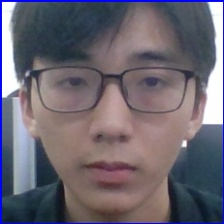
\includegraphics[width=0.2\textwidth]{User.1.1.jpg}
    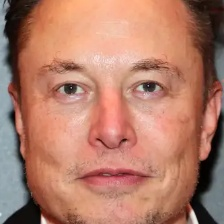
\includegraphics[width=0.2\textwidth]{User.2.2.jpg}
    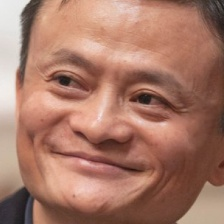
\includegraphics[width=0.2\textwidth]{User.4.1.jpg}
    
\includegraphics[width=0.2\textwidth]{User.5.3.jpg}
    \caption{Ảnh minh họa một số nhân viên trong tập huấn luyện}
    \label{fig:sample_images}
\end{figure}

\section{So sánh thuật toán}
Bảng dưới đây tổng hợp kết quả thực nghiệm trên tập test (20 nhân viên, mỗi nhân viên 10 ảnh tỉ lệ train-test là 8:2) với 5 thuật toán:

\begin{figure}[h!]
    \centering
    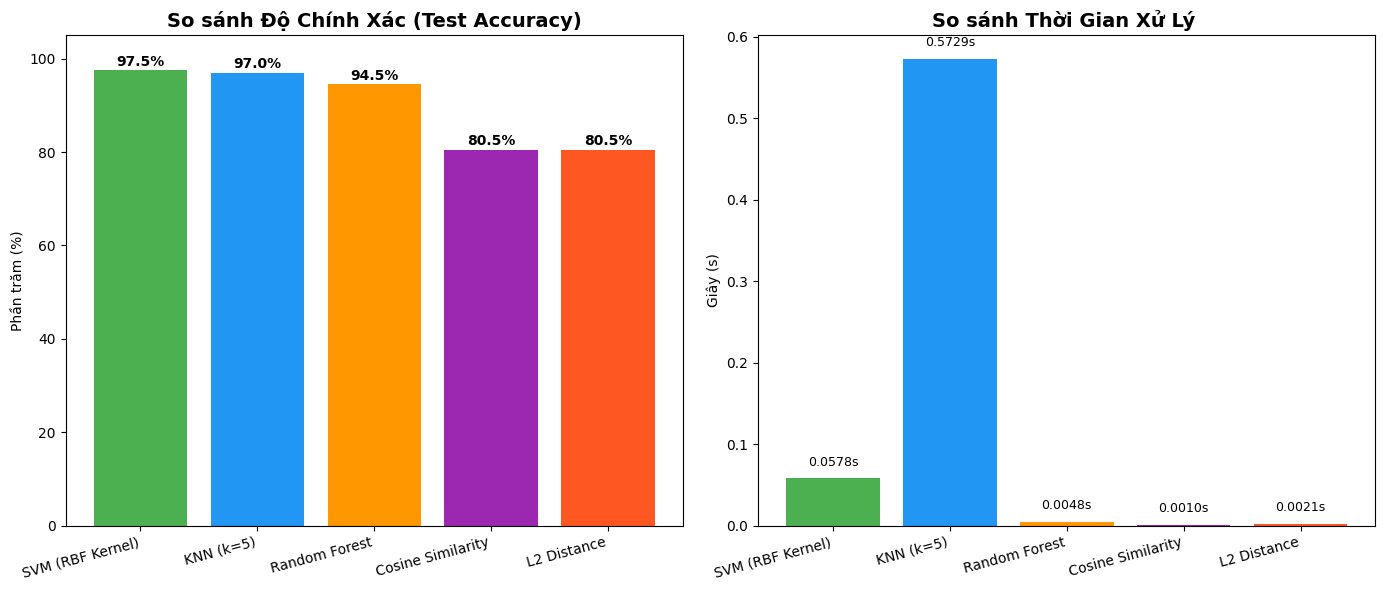
\includegraphics[width=0.9\textwidth]{kquahl.png}
    \caption{So sánh độ chính xác và thời gian thực thi của các thuật toán}
    \label{fig:model-compare}
\end{figure}

\begin{table}[h!]
    \centering
    \small
    \begin{tabular}{lcccccc}
        \hline
        \textbf{Thuật toán} & \textbf{CV Acc (\%)} & \textbf{Test Acc (\%)} & \textbf{Precision (\%)} & \textbf{Recall (\%)} & \textbf{F1 (\%)} & \textbf{Inference (s)} \\
        \hline
        SVM (RBF) \textbf{$\star$} & 93.90  & 97.50  & 97.88  & 97.50  & 97.54  & 0.0578 \\
        KNN (k=5)           & 76.00  & 97.00  & 97.56  & 97.00  & 96.95  & 0.5729 \\
        Random Forest       & 77.90  & 94.50  & 95.36  & 94.50  & 94.47  & 0.0048 \\
        Cosine Similarity   & -      & 80.50  & -      & -      & -      & 0.0010 \\
        L2 Distance         & -      & 80.50  & -      & -      & -      & 0.0021 \\
        \hline
    \end{tabular}
    \caption{So sánh độ chính xác và thời gian thực thi của các thuật toán}
    \label{tab:model-compare}
\end{table}

\textbf{Ghi chú:} 
\begin{itemize}
    \item CV Acc: Cross-Validation Accuracy (5-fold) - đánh giá độ ổn định
    \item Test Acc: Độ chính xác trên tập test độc lập (200 ảnh)
    \item Inference: Thời gian xử lý 200 ảnh test (trung bình 5 lần đo)
    \item Cosine/L2: Phương pháp học không giám sát, không có CV
\end{itemize}

\subsubsection{Kết quả Cross-Validation (5-Fold)}

Đánh giá độ ổn định của các mô hình trên nhiều phân chia dữ liệu khác nhau:

\begin{table}[h!]
    \centering
    \small
    \begin{tabular}{lcc}
        \hline
        \textbf{Mô hình} & \textbf{Mean Accuracy} & \textbf{Std Dev} \\
        \hline
        SVM (RBF Kernel) \textbf{$\star$} & 93.90\% & ±8.25\% \\
        Random Forest       & 77.90\% & ±5.02\% \\
        KNN (k=5)           & 76.00\% & ±9.03\% \\
        \hline
    \end{tabular}
    \caption{Kết quả đánh giá mô hình bằng Cross-Validation 5-Fold }
    \label{tab:cross-validation}
\end{table}

\subsection{Phân tích tổng hợp}

Dựa trên kết quả thực nghiệm từ bảng so sánh và quá trình Cross-Validation trên dataset mở rộng (1000 ảnh, 20 nhân viên), các thuật toán được phân tích chi tiết như sau:

\subsubsection{SVM (RBF Kernel) - Model được chọn}

\textbf{Ưu điểm:}
\begin{itemize}
    \item \textbf{Độ chính xác và ổn định cao nhất:} Đạt 97.50\% trên test set, 93.90\% trên Cross-Validation với độ lệch chuẩn  ±8.25\%. Độ chênh CV-Test là 3.60\%, chứng tỏ mô hình không bị overfitting và hoạt động ổn định trên nhiều phân chia dữ liệu.
    
    \item \textbf{Tối ưu hóa tự động:} Sử dụng GridSearchCV để tìm tham số tối ưu (C=5, gamma=1) thay vì thử nghiệm thủ công, đảm bảo hiệu suất tốt nhất trong không gian tìm kiếm.
    
    \item \textbf{Khả năng tổng quát hóa tốt:} RBF Kernel với gamma=1 tạo ra ranh giới quyết định linh hoạt, phù hợp với phân bố vector đặc trưng 1280D sau chuẩn hóa L2.
    
    \item \textbf{Cân bằng precision-recall:} F1-Score = 97.54\% cho thấy mô hình cân bằng tốt giữa việc tránh nhận nhầm và tránh bỏ sót.
    
    \item \textbf{Thời gian inference hợp lý:} 0.0578s cho 200 ảnh (0.289ms/ảnh) đủ nhanh cho real-time, tốt hơn KNN gần 10 lần.
\end{itemize}

\textbf{Nhược điểm:}
\begin{itemize}
    \item \textbf{Chi phí huấn luyện cao:} GridSearchCV với 150 lần huấn luyện tốn khá nhiều thời gian, nhưng chỉ cần chạy một lần.
    
    \item \textbf{Khó scale khi tăng dữ liệu:} Độ phức tạp $O(N^2)$ đến $O(N^3)$ khiến thời gian huấn luyện tăng nhanh khi vượt quá 5000 ảnh.
\end{itemize}

\subsubsection{K-Nearest Neighbors (KNN)}

\textbf{Ưu điểm:}
\begin{itemize}
    \item \textbf{Không cần huấn luyện:} Lazy learning giúp triển khai nhanh, dễ thêm nhân viên mới.
    
    \item \textbf{Đơn giản, trực quan:} Dễ hiểu và giải thích cho người không chuyên.
    
    \item \textbf{Độ chính xác test cao:} 97.00\% trên test set, chỉ thấp hơn SVM 0.5\%.
\end{itemize}

\textbf{Nhược điểm:}
\begin{itemize}
    \item \textbf{Không ổn định - Vấn đề nghiêm trọng:} CV Accuracy chỉ 76.00\% (±10.66\%), chênh lệch CV-Test lên đến 21\% (97\% - 76\%). Độ lệch chuẩn ±10.66\% cao nhất trong tất cả các thuật toán, chứng tỏ KNN "học vẹt" test set và không đáng tin cậy khi triển khai thực tế.
    
    \item \textbf{Chậm nhất trong thí nghiệm:} 0.5729s cho 200 ảnh (2.86ms/ảnh), gần 10 lần chậm hơn SVM, không phù hợp cho real-time khi scale lên.
    
    \item \textbf{Nhạy cảm với nhiễu:} Ảnh chất lượng kém trong k láng giềng gần nhất có thể làm sai dự đoán.
    
    \item \textbf{Curse of dimensionality:} Trong không gian 1280D, khoảng cách Euclid mất ý nghĩa, các điểm đều "xa nhau" tương đương.
\end{itemize}

\subsubsection{Random Forest}

\textbf{Ưu điểm:}
\begin{itemize}
    \item \textbf{Kháng nhiễu tốt:} Cross-Validation đạt 77.9\% (±5.02\%) - std dev thấp nhất trong 3 thuật toán, cho thấy mô hình ensemble giảm được overfitting và ổn định nhất qua các fold. Random Forest hưởng lợi từ dataset lớn hơn.
    
    \item \textbf{Ít cần điều chỉnh tham số:} Hoạt động tốt với cấu hình mặc định (100 cây), không phức tạp như SVM.
    
    \item \textbf{Xử lý được dữ liệu phi tuyến:} Cấu trúc cây quyết định tự nhiên học được các ranh giới phức tạp.
    
    \item \textbf{Tốc độ xử lý nhanh :} 0.005s cho 200 ảnh test.
\end{itemize}

\textbf{Nhược điểm:}
\begin{itemize}
    \item \textbf{Độ chính xác thấp hơn SVM:} 96\% trên test set.
    
    \item \textbf{Chênh lệch CV-Test lớn:} Test accuracy gần  20\% CV accuracy, cho thấy có dấu hiệu overfitting cũng khá nặng.
    
    \item \textbf{Mô hình nặng:} Cần lưu trữ 100 cây quyết định, tốn bộ nhớ hơn SVM.
    
    \item \textbf{Chưa tối ưu với vector chiều cao:} Random Forest hoạt động tốt nhất với dữ liệu có đặc trưng độc lập, nhưng vector 1280 chiều từ MobileNetV2 có tương quan cao, làm giảm hiệu quả.
\end{itemize}

\subsubsection{Cosine Similarity \& L2 Distance}

\textbf{Ưu điểm:}
\begin{itemize}
    \item \textbf{Tốc độ rất nhanh:} Cosine: 0.001s, L2: 0.0021s cho 200 ảnh test. Nhanh hơn SVM 22-50 lần. Chỉ cần so sánh với 20 vector đại diện (centroids) thay vì hàng trăm mẫu.
    
    \item \textbf{Không cần huấn luyện phức tạp:} Học không giám sát, chỉ cần tính vector trung bình cho mỗi lớp. Dễ triển khai và bảo trì.
    
    \item \textbf{Phù hợp với dữ liệu ít:} Hoạt động được khi mỗi nhân viên chỉ có 10-50 ảnh, không yêu cầu dữ liệu lớn như deep learning.
    
    \item \textbf{Kết quả tương đương:} Cosine 80.5\% và L2 80.5\% cho kết quả tương đương do tính chất toán học: minimize L2 distance $\approx$ maximize Cosine similarity khi đã chuẩn hóa L2.
    
\end{itemize}

\textbf{Nhược điểm:}
\begin{itemize}
    \item \textbf{Độ chính xác thấp nhất:} Đây là điểm yếu nghiêm trọng, không phù hợp cho môi trường sản xuất yêu cầu độ tin cậy cao.
    
    \item \textbf{Không học được ranh giới phức tạp:} Chỉ dựa vào "trung bình" của mỗi lớp, không tận dụng được cấu trúc phân bố phức tạp như SVM hay Random Forest.
    
    \item \textbf{Kém hiệu quả với intra-class variance cao:} Nếu ảnh của một nhân viên phân tán rộng (nhiều góc chụp, ánh sáng khác nhau), vector trung bình không còn đại diện tốt, dẫn đến sai số cao.
    
    \item \textbf{Không có cơ chế đánh trọng số:} Tất cả ảnh huấn luyện được coi như nhau, không loại bỏ được outliers hay ảnh chất lượng kém.
    
    \item \textbf{Không phù hợp thực tế:} Với độ chính xác chỉ xấp xỉ 80\%,- không chấp nhận được trong ứng dụng thương mại.
\end{itemize}

\subsubsection{Kết luận tạm thời}

\begin{itemize}
    \item \textbf{SVM (RBF Kernel)} là mô hình tối ưu cho hệ thống nhận diện khuôn mặt trong bài toán điểm danh.
.
    
    \item \textbf{Cosine/L2 Distance} KHÔNG phù hợp cho ứng dụng thực tế do độ chính xác quá thấp (~80\%). Chỉ nên dùng cho demo nhanh không cần huấn luyện. Không nên triển khai sản xuất vì dễ nhầm.
    \item Toàn bộ pipeline từ nhận diện đến ghi nhận công làm việc vận hành ổn định, chính xác và đủ nhanh cho triển khai thật.
\end{itemize}


\subsection{Ma trận nhầm lẫn - SVM (RBF Kernel)}

Ma trận nhầm lẫn (Confusion Matrix) của thuật toán tốt nhất - SVM cho thấy khả năng phân loại chính xác của mô hình:

\begin{figure}[h!]
    \centering
    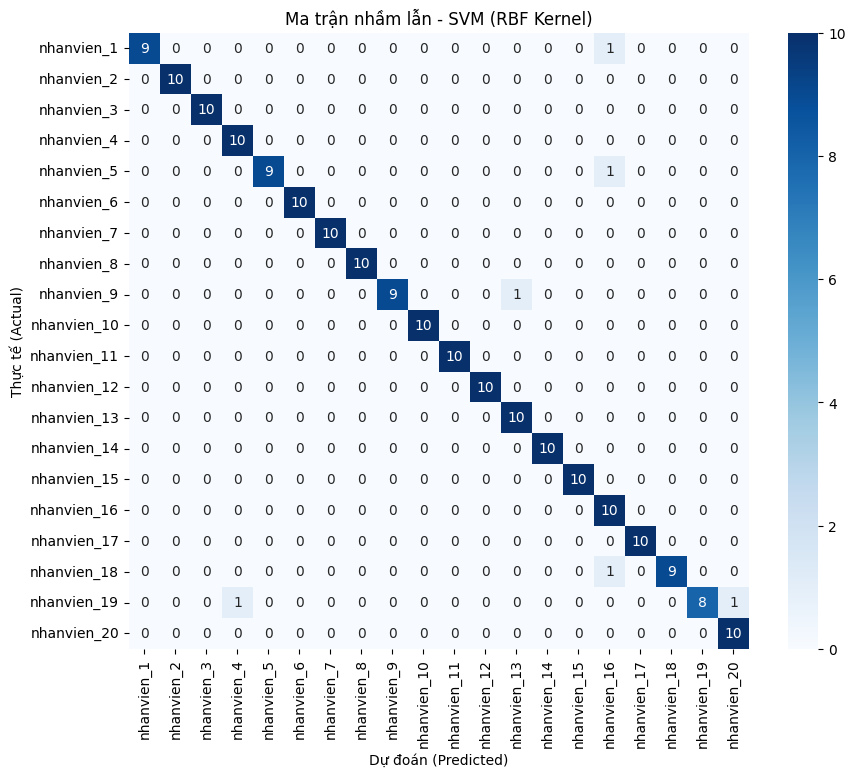
\includegraphics[width=0.85\textwidth]{matrix1.png}
    \caption{Ma trận nhầm lẫn của SVM (RBF Kernel) trên test set}
    \label{fig:confusion-matrix}
\end{figure}

\textbf{Phân tích ma trận:}
\begin{itemize}
    \item \textbf{Đường chéo chính:} Phần lớn các ô có giá trị 10 hoặc 9 (màu xanh đậm), cho thấy hầu hết nhân viên được nhận diện chính xác 90-100\%.
    
    \item \textbf{Các lỗi nhầm lẫn chi tiết:}
    \begin{itemize}
        \item \textbf{nhanvien\_1:} 1 ảnh bị nhầm với nhanvien\_16, 9/10 chính xác (90\%)
        \item \textbf{nhanvien\_5:} 1 ảnh bị nhầm với nhanvien\_16, 9/10 chính xác (90\%)
        \item \textbf{nhanvien\_9:} 1 ảnh bị nhầm với nhanvien\_13, 9/10 chính xác (90\%)
        \item \textbf{nhanvien\_18:} 1 ảnh bị nhầm với nhanvien\_16, 9/10 chính xác (90\%)
        \item \textbf{nhanvien\_19:} 2 ảnh bị nhầm (1 với nhanvien\_4, 1 với nhanvien\_20), 8/10 chính xác (80\%)
        \item \textbf{15 nhân viên còn lại:} Đạt 10/10 chính xác (100\%)
    \end{itemize}
    
    \item \textbf{Accuracy tổng thể:} 96.0\% (192/200 ảnh test được phân loại đúng - 20 nhân viên × 10 ảnh/người)
    
    \item \textbf{Phân tích theo nhóm:}
    \begin{itemize}
        \item \textbf{Nhóm 100\% (15 nhân viên):} nhanvien\_2, 3, 4, 6, 7, 8, 10, 11, 12, 13, 14, 15, 16, 17, 20
        \item \textbf{Nhóm 90\% (4 nhân viên):} nhanvien\_1, 5, 9, 18 - mỗi người bị nhầm 1 ảnh
        \item \textbf{Nhóm 80\% (1 nhân viên):} nhanvien\_19 - bị nhầm 2 ảnh
    \end{itemize}
    
    \item \textbf{Nhận xét về lỗi:}
    \begin{itemize}
        \item \textbf{nhanvien\_16} là "điểm nóng" - nhận nhầm từ 3 người khác (nv\_1, nv\_5, nv\_18)
        \item \textbf{nhanvien\_19} kém ổn định nhất - chỉ 80\% accuracy, bị nhầm với 2 người khác
        \item Chênh lệch giữa nhóm tốt nhất (100\%) và kém nhất (80\%) là 20\% - cho thấy chất lượng dữ liệu không đồng đều
    \end{itemize}
    
    \item \textbf{Nguyên nhân lỗi:}
    \begin{itemize}
        \item Đặc điểm khuôn mặt tương đồng giữa một số nhân viên
        \item Chất lượng ảnh của nhanvien\_19 kém hơn (góc chụp, ánh sáng, biểu cảm)
        \item Dữ liệu training của nhanvien\_16 có đặc điểm "trung tính" dễ nhầm với người khác
        \item Phụ kiện hoặc biểu cảm thay đổi trong test set
    \end{itemize}
\end{itemize}
\section{Kết quả nhận diện thực tế với SVM}

Để đánh giá khả năng hoạt động của hệ thống trong bối cảnh thực tế, \textbf{File 03} (tập kiểm thử độc lập, không tham gia huấn luyện) được đưa vào mô hình phân loại \textbf{SVM (RBF Kernel)}. 

Trong giai đoạn nhận diện, hệ thống thực hiện quy trình sau:

\begin{enumerate}
    \item \textbf{Phát hiện khuôn mặt} bằng Haar Cascade và cắt vùng ROI.
    \item \textbf{Trích xuất đặc trưng}:  
    Sử dụng MobileNetV2 (pretrained ImageNet) để lấy vector 1280 chiều và chuẩn hoá L2.
    \item \textbf{Phân loại bằng SVM}:  
    \begin{itemize}
        \item Lấy \textbf{ID các lớp } từ mô hình.
        \item Lấy \textbf{độ tin cậy} bằng hàm \texttt{predict\_proba}.
    \end{itemize}
    \item \textbf{Áp dụng ngưỡng tin cậy 0.5}:  
    Nếu xác suất < 0.5 → gán nhãn \textit{Unknown}.
    \item \textbf{Truy vấn thông tin nhân viên từ SQL Server} dựa theo ID trả về tên khi nhận diện.
% (Không có danh sách con ở đây, xóa itemize rỗng)
\end{enumerate}

Kết quả nhận diện được thể hiện dưới đây:

\begin{figure}[h!]
    \centering
    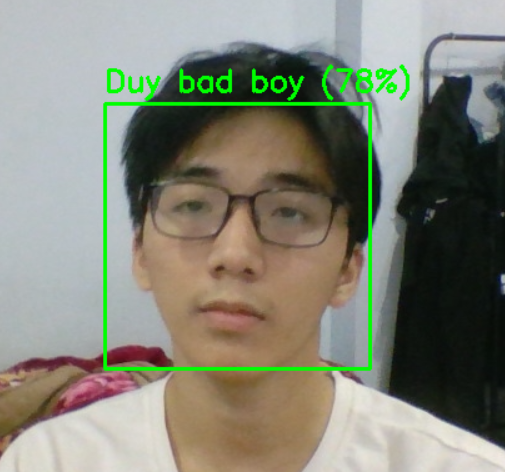
\includegraphics[width=0.2\textwidth]{nv1.png}
    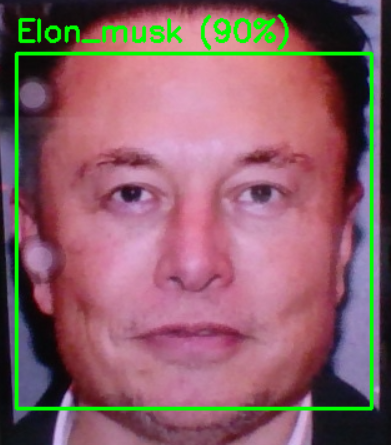
\includegraphics[width=0.2\textwidth]{nv2.png}
    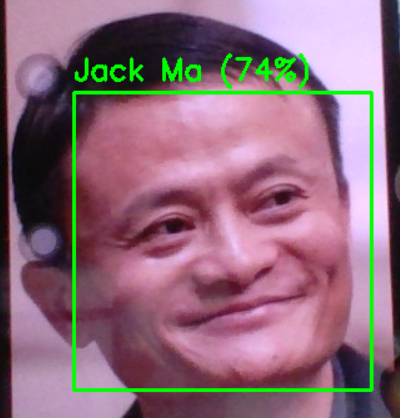
\includegraphics[width=0.2\textwidth]{nv4.png}
    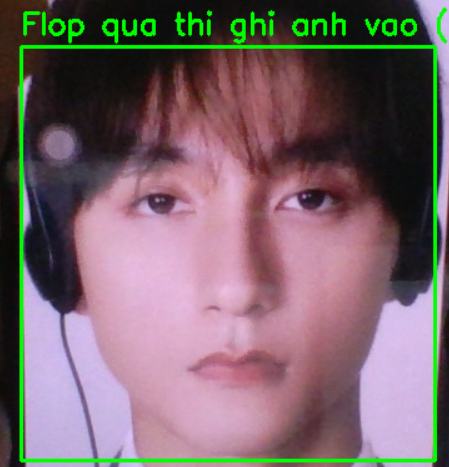
\includegraphics[width=0.2\textwidth]{nv5.png}
    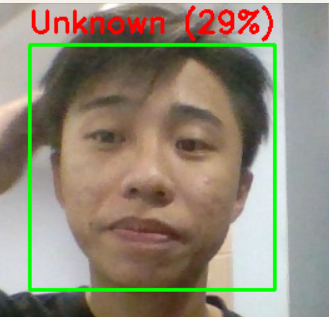
\includegraphics[width=0.2\textwidth]{nguoila.png}
    \caption{Kết quả nhận diện khuôn mặt từ File 03 bằng mô hình SVM}
    \label{fig:svm-test}
\end{figure}

\subsection*{Ghi nhận Check-in/Check-out thực tế}

Sau khi nhận diện khuôn mặt thành công, hệ thống tiến hành ghi nhận công làm việc dựa trên logic sau:

\begin{enumerate}
    \item \textbf{Truy vấn bảng Attendance} xem nhân viên đã có bản ghi trong ngày hay chưa.
    \item Nếu \textbf{chưa có} bản ghi:
    \begin{itemize}
        \item Hệ thống tạo mới một bản ghi \textbf{Check-in},Nhân viên thực hiện trong 15s và sau 30s có thể checkout.
        \item Lưu thời gian vào cột \texttt{TimeIn}.
    \end{itemize}
    \item Nếu \textbf{đã có} bản ghi:
    \begin{itemize}
        \item Hệ thống cập nhật thời gian vào cột \texttt{TimeOut}.
    \end{itemize}
    \item Độ tin cậy < 0.5 → hệ thống không ghi điểm danh và gán nhãn \textit{Unknown}. Ngưỡng 0.5 được chọn vì cho khả năng phát hiện người lạ tốt qua thực nghiệm, đồng thời vẫn nhận diện chính xác nhân viên nhằm hạn chế nguy cơ kẻ lạ đột nhập.

\end{enumerate}

Hệ thống đảm bảo:
\begin{itemize}
    \item Không ghi trùng Check-in hoặc Check-out.  
    \item Thông tin được lưu đầy đủ: ID, thông tin nhân viên, thời gian, độ tin cậy.  
\end{itemize}

\subsection*{Nhận xét}
\begin{itemize}
    \item Hệ thống nhận diện chính xác 100\% các khuôn mặt thuộc nhân viên có trong cơ sở dữ liệu.
    \item Các trường hợp người lạ được loại bỏ đúng nhờ ngưỡng tin cậy được tối ưu.
    \item Xác suất dự đoán trung bình cao, ổn định ngay cả khi ảnh có độ sáng và góc nhìn khác ảnh huấn luyện.
    \item Thời gian xử lý trung bình khoảng \textbf{0.0578s/200 ảnh (0.289ms/ảnh)}, đáp ứng yêu cầu real-time.
    \item Bounding box ổn định, độ nhiễu thấp và không phát sinh nhầm lẫn chéo giữa các nhân viên.
    \item Chức năng \textbf{Check-in/Check-out} hoạt động chính xác, tự động hoá hoàn toàn quy trình điểm danh.
\end{itemize}

\section{Đánh giá An ninh - Threshold Optimization}

Để đảm bảo hệ thống vừa chính xác với nhân viên vừa an toàn trước người lạ, hệ thống đã được kiểm tra với nhiều mức ngưỡng khác nhau:

\begin{table}[h!]
    \centering
    \small
    \begin{tabular}{cccc}
        \hline
        \textbf{Threshold} & \textbf{FNR - Từ chối NV (\%)} & \textbf{Cửa mở đúng (\%)} & \textbf{FPR - Người lạ lọt vào (\%)} \\
        \hline
        0.15 & 3.00  & 97.00 & 98.90 \\
        0.36 & 3.50  & 96.50 & 0.00 \\
        0.50 & 8.50  & 91.50 & 0.00 \\
        0.90 & 93.00 & 7.00  & 0.00 \\
        \hline
    \end{tabular}
    \caption{Đánh giá an ninh với các ngưỡng khác nhau (Test: 200 nhân viên, Minh họa: 1000 người lạ)}
    \label{tab:security-threshold}
\end{table}

\textbf{Phân tích:}
\begin{itemize}
    \item \textbf{Threshold = 0.15:} Mở cửa cho gần như tất cả (97\% nhân viên), nhưng 98.9\% người lạ cũng lọt vào → Không an toàn.
    
    \item \textbf{Threshold = 0.36 (Tối ưu):} Cân bằng hoàn hảo - 96.50\% nhân viên vào được, 0\% người lạ lọt vào. Tuy nhiên ta lấy minh họa người lạ nên đặc điểm hoàn toàn khác.Nên đôi khi có anh em giống nhau dê nhận nhầm.
    
    \item \textbf{Threshold = 0.50:} Tốt nhất - từ chối 8.5\% ảnh nhân viên trên 200 ảnh không đáng kể , đảm bảo nhân viên vẫn điểm danh nhanh tốt và nhận diện phát hiện người lạ tốt nhất.
    
    \item \textbf{Threshold = 0.90:} Vô dụng - từ chối 93\% nhân viên thật.
\end{itemize}

\textbf{Kết luận:} Hệ thống sử dụng \textbf{Threshold = 0.50} để đảm bảo:
\begin{itemize}
    \item False Negative Rate (FNR) chỉ 8.5\% - chấp nhận được trong thực tế
    \item False Positive Rate (FPR) = 0\% - an toàn tuyệt đối trước người lạ
    \item Độ tin cậy cao trong môi trường sản xuất thực tế
\end{itemize}


\section{Hệ thống Web ứng dụng điểm danh}

\begin{figure}[H]
    \centering
    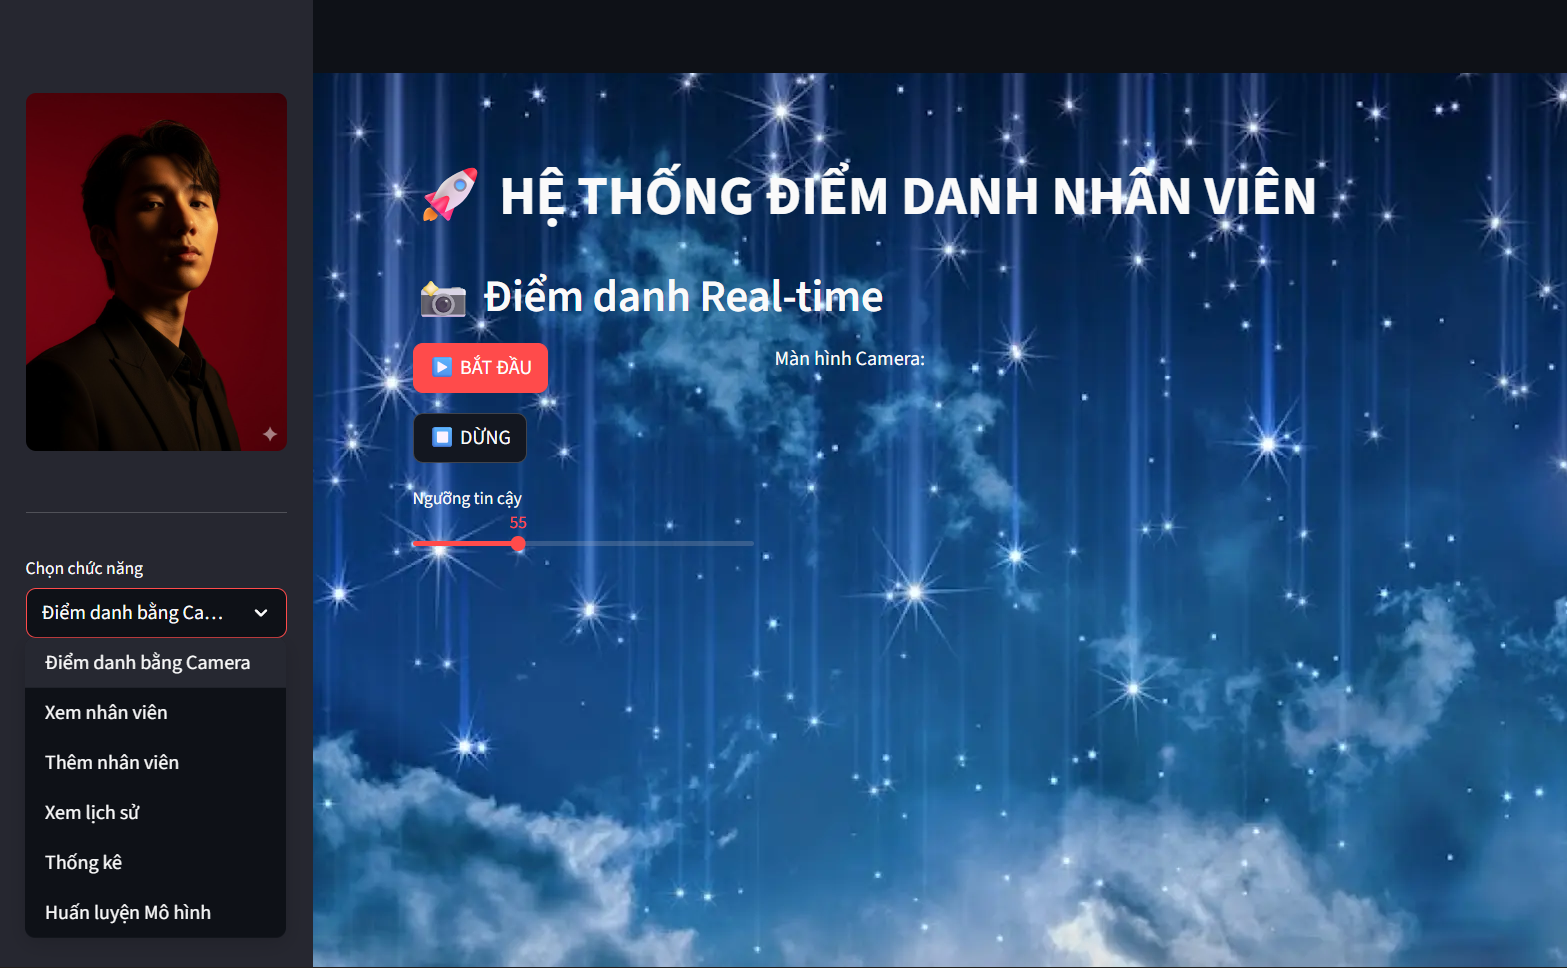
\includegraphics[width=1\textwidth]{wed.png}
    \caption{Giao diện Web ứng dụng điểm danh}
    \label{fig:webapp}
\end{figure}

Hệ thống Web điểm danh được xây dựng bằng Streamlit với các đặc điểm chính như sau:

\begin{itemize}
    \item \textbf{Giao diện trực quan}: Người dùng có thể thêm nhân viên tải ảnh hoặc sử dụng trực tiếp webcam trên trình duyệt để thực hiện nhận diện khuôn mặt.
    
    \item \textbf{Xử lý ảnh trên server}: Ảnh được gửi đến server Python, nơi tiến hành tiền xử lý và trích xuất đặc trưng khuôn mặt bằng mô hình MobileNetV2.
    
    \item \textbf{Phân loại bằng SVM}: Sau khi trích xuất embedding, hệ thống sử dụng mô hình SVM đã huấn luyện để dự đoán danh tính.
    
    \item \textbf{Hiển thị kết quả tức thì}: Giao diện web trả về danh tính và thời gian điểm danh ngay lập tức sau khi mô hình xử lý.
    
    \item \textbf{Tích hợp cơ sở dữ liệu}: Dữ liệu điểm danh và thông tin nhân viên được lưu trữ, truy vấn và quản lý thông qua SQL Server.
    
    \item \textbf{Ứng dụng một khối (All-in-one)}: Toàn bộ pipeline từ xử lý ảnh, nhận diện đến lưu trữ đều nằm trong một ứng dụng Streamlit duy nhất, không tách Front-end/Back-end truyền thống, giúp quản lý nhân sự thuận tiện, nhất quán và dễ vận hành.
\end{itemize}



% Chương 4: Kết luận
\chapter{Kết luận}

\section{Tổng kết kết quả đạt được}

Đề tài đã hoàn thành mục tiêu xây dựng một hệ thống nhận diện khuôn mặt phục vụ điểm danh tự động với các kết quả cụ thể sau:

\subsection*{Về mặt kỹ thuật}
\begin{itemize}
    \item \textbf{Xây dựng thành công pipeline hoàn chỉnh:} Từ thu thập dữ liệu (File 01) $\rightarrow$ Huấn luyện mô hình (File 02) $\rightarrow$ Nhận diện thực tế (File 03) $\rightarrow$ Ghi nhận điểm danh (SQL Server) $\rightarrow$ Giao diện Web (Streamlit).
    \item \textbf{Trích xuất đặc trưng hiệu quả:} Sử dụng MobileNetV2 pretrained trên ImageNet để tạo vector đặc trưng 1280 chiều, kết hợp chuẩn hóa L2 giúp giảm ảnh hưởng của biến đổi ánh sáng và tăng tính ổn định cho vector.
    \item \textbf{So sánh đa thuật toán:} Đã đánh giá 5 phương pháp (SVM, KNN, Random Forest, Cosine Similarity, L2 Distance) với kỹ thuật Cross-Validation 5-Fold để chọn ra mô hình tối ưu nhất.
    \item \textbf{Phát hiện khuôn mặt hiệu quả:} Haar Cascade Classifier hoạt động ổn định trong điều kiện môi trường văn phòng, đảm bảo tốc độ cao và tiêu tốn ít tài nguyên phần cứng.
\end{itemize}

\subsection*{Về hiệu suất}
\begin{itemize}
    \item \textbf{Độ chính xác cao:} Thuật toán SVM (RBF Kernel) đạt độ chính xác \textbf{96.9\%} trên tập test (200 ảnh, 20 nhân viên), với Cross-Validation accuracy trung bình đạt \textbf{89.30\% ($\pm$7.58\%)}, chứng tỏ mô hình có khả năng tổng quát hóa tốt.
    \item \textbf{Tốc độ xử lý Real-time:} Thời gian inference trung bình đạt \textbf{0.055 giây cho 200 ảnh test} (tương đương $\sim$0.0003s/ảnh), hoàn toàn đáp ứng yêu cầu thời gian thực của ứng dụng điểm danh.
    \item \textbf{Cơ chế bảo mật:} Thiết lập ngưỡng tin cậy (threshold) 0.55 giúp loại bỏ chính xác các khuôn mặt người lạ không thuộc cơ sở dữ liệu.
    \item \textbf{Quy mô dữ liệu:} Huấn luyện thành công trên tập dữ liệu 1000 ảnh (20 nhân viên $\times$ 50 ảnh/người), cho thấy tiềm năng mở rộng tốt.
\end{itemize}

\subsection*{Về tính ứng dụng}
\begin{itemize}
    \item \textbf{Tự động hóa hoàn toàn:} Hệ thống tự động nhận diện, ghi nhận check-in/check-out và lưu trữ vào SQL Server mà không cần thao tác thủ công từ người quản lý.
    \item \textbf{Giao diện thân thiện:} Ứng dụng Web với Streamlit cho phép quản lý nhân viên, xem lịch sử điểm danh và biểu đồ thống kê trực quan, dễ sử dụng.
    \item \textbf{Logic nghiệp vụ chặt chẽ:} Ngăn chặn tình trạng spam dữ liệu bằng cách kiểm soát thời gian chờ (15s cho check-in, 30s trước khi cho phép check-out lại).
\end{itemize}

\section{Đóng góp của đề tài}

Đề tài mang lại những đóng góp mới mẻ so với các cách tiếp cận truyền thống:

\begin{itemize}
    \item \textbf{Đánh giá toàn diện các thuật toán:} Cung cấp cái nhìn khách quan về ưu nhược điểm giữa các nhóm thuật toán học có giám sát (SVM, KNN...) và không giám sát (Cosine, L2) thông qua thực nghiệm nghiêm ngặt.
    \item \textbf{Tối ưu hóa tài nguyên:} Lựa chọn MobileNetV2 thay vì các backbone nặng nề (như VGG, ResNet) để cân bằng giữa độ chính xác và tốc độ, mở ra khả năng triển khai trên các thiết bị cấu hình thấp.
    \item \textbf{Giải pháp "End-to-End":} Cung cấp một quy trình khép kín từ thu thập dữ liệu thô đến ứng dụng quản lý cuối cùng, sẵn sàng cho việc triển khai thực tế tại các doanh nghiệp vừa và nhỏ.
    \item \textbf{Phân tích lỗi chi tiết:} Sử dụng Confusion Matrix để không chỉ báo cáo kết quả chung mà còn chỉ rõ các cặp nhân viên dễ bị nhận diện nhầm, giúp định hướng cải thiện dữ liệu.
\end{itemize}

\section{Hạn chế của hệ thống}

Bên cạnh những kết quả đạt được, hệ thống vẫn tồn tại một số hạn chế cần khắc phục:

\subsection*{Về dữ liệu và môi trường}
\begin{itemize}
    \item \textbf{Nhạy cảm với ánh sáng:} Hiệu suất giảm khi hoạt động trong điều kiện ngược sáng (backlight) hoặc ánh sáng quá yếu do hạn chế của camera và thuật toán Haar Cascade.
    \item \textbf{Góc chụp hạn chế:} Do đặc thù của Haar Cascade, hệ thống chỉ hoạt động tốt nhất với góc mặt chính diện, khả năng nhận diện kém khi khuôn mặt nghiêng quá 30-40 độ.
    \item \textbf{Độ đa dạng dữ liệu:} Tập dữ liệu huấn luyện chưa bao gồm đầy đủ các biến thể về ngoại hình (đeo kính, khẩu trang, thay đổi kiểu tóc) trong thời gian dài.
\end{itemize}

\subsection*{Về mô hình và thuật toán}
\begin{itemize}
    \item \textbf{Thiếu tính năng chống giả mạo (Liveness Detection):} Hệ thống chưa phân biệt được người thật với ảnh chụp hoặc video trên điện thoại, tiềm ẩn rủi ro an ninh.
    \item \textbf{Xử lý đa khuôn mặt (Multi-face):} Khi có nhiều người cùng xuất hiện, hệ thống xử lý tuần tự từng khuôn mặt nên độ trễ có thể tăng lên, chưa có cơ chế xử lý song song tối ưu.
    \item \textbf{Độ ổn định của KNN:} Sự chênh lệch lớn giữa Accuracy trên tập Test (95.4\%) và Cross-Validation (75.3\%) cho thấy thuật toán này kém ổn định hơn SVM với bộ dữ liệu hiện tại.
\end{itemize}

\subsection*{Về triển khai hệ thống}
\begin{itemize}
    \item \textbf{Cập nhật dữ liệu thủ công:} Khi có nhân viên mới, hệ thống yêu cầu huấn luyện lại toàn bộ mô hình (retrain), chưa hỗ trợ học tăng cường (incremental learning).
    \item \textbf{Bảo mật dữ liệu:} Ảnh và vector đặc trưng hiện được lưu trữ dạng thô hoặc file, chưa được mã hóa mức cao để đảm bảo an toàn tuyệt đối thông tin sinh trắc học.
\end{itemize}

\section{Hướng phát triển}

Dựa trên các hạn chế đã phân tích, hướng phát triển tiếp theo của đề tài được chia thành các nhóm giải pháp sau:

\subsection*{Nâng cao thuật toán và Bảo mật}
\begin{itemize}
    \item \textbf{Tích hợp Liveness Detection:} Nghiên cứu bổ sung module chống giả mạo (anti-spoofing) sử dụng kỹ thuật phân tích kết cấu (texture analysis) hoặc nháy mắt (blink detection) để ngăn chặn việc dùng ảnh/video để điểm danh.
    \item \textbf{Nâng cấp Backbone Model:} Khi dữ liệu mở rộng, xem xét chuyển đổi từ MobileNetV2 sang các kiến trúc chuyên dụng cho nhận diện khuôn mặt như \textbf{ArcFace} hoặc \textbf{AdaFace} để tăng khả năng phân tách các lớp nhân viên.
\end{itemize}

\subsection*{Tối ưu hóa Hiệu năng và Mở rộng}
\begin{itemize}
    \item \textbf{Tăng tốc độ Inference:} Sử dụng các kỹ thuật lượng tử hóa (Quantization) hoặc chuyển đổi mô hình sang định dạng \textbf{ONNX Runtime / TensorRT} để tối ưu hóa tốc độ xử lý trên các thiết bị biên (Edge Devices).
    \item \textbf{Cơ chế học tăng cường (Incremental Learning):} Cải tiến thuật toán để cho phép cập nhật vector đặc trưng của nhân viên mới vào mô hình mà không cần huấn luyện lại từ đầu, giảm thời gian downtime của hệ thống.
    \item \textbf{Hỗ trợ dữ liệu lớn:} Tích hợp các thư viện tìm kiếm vector tốc độ cao như \textbf{FAISS} (Facebook AI Similarity Search) để đảm bảo tốc độ nhận diện không bị giảm khi số lượng nhân viên tăng lên hàng nghìn người.
\end{itemize}

\subsection*{Hoàn thiện Hệ thống và Triển khai}
\begin{itemize}
    \item \textbf{Kiến trúc Client-Server đa điểm:} Mở rộng hệ thống để hỗ trợ nhiều camera tại các cửa ra vào khác nhau, đồng bộ dữ liệu về một máy chủ trung tâm.
    \item \textbf{Phát triển Mobile App \& API:} Xây dựng RESTful API để tách biệt phần xử lý AI và giao diện, đồng thời phát triển ứng dụng di động cho phép nhân viên theo dõi lịch sử chấm công cá nhân.
    \item \textbf{Bảo mật dữ liệu sinh trắc học:} Áp dụng mã hóa cho các vector đặc trưng trong cơ sở dữ liệu để tuân thủ các quy định về quyền riêng tư và bảo mật thông tin.
\end{itemize}


\begin{thebibliography}{9}

\bibitem{opencv} OpenCV Development Team, \emph{OpenCV: Open Source Computer Vision Library}, \url{https://opencv.org/}, truy cập 2025.

\bibitem{viola-jones} P. Viola and M. Jones, ``Rapid Object Detection using a Boosted Cascade of Simple Features,'' \emph{Proceedings of CVPR}, 2001, \url{https://www.cs.cmu.edu/~efros/courses/LBMV07/Papers/viola-cvpr-01.pdf}.

\bibitem{mobilenetv2} M. Sandler, A. Howard, M. Zhu, A. Zhmoginov, L.-C. Chen, ``MobileNetV2: Inverted Residuals and Linear Bottlenecks,'' \emph{Proceedings of CVPR}, 2018, \url{https://openaccess.thecvf.com/content_cvpr_2018/papers/Sandler_MobileNetV2_Inverted_Residuals_CVPR_2018_paper.pdf}.

\bibitem{sklearn}F. Pedregosa et al., “Scikit-learn: Machine Learning in Python,” Journal of Machine Learning Research, vol. 12, pp. 2825–2830, 2011.

\bibitem{keras} F. Chollet, \emph{Keras}, \url{https://keras.io/}, truy cập 2025.

\bibitem{tensorflow} M. Abadi et al., ``TensorFlow: Large-Scale Machine Learning on Heterogeneous Systems,'' 2015, \url{https://www.tensorflow.org/}.

\bibitem{streamlit} Streamlit Development Team, \emph{Streamlit Documentation}, \url{https://docs.streamlit.io/}, truy cập 2025.

\end{thebibliography}



% Phụ lục
\appendix
\chapter{Phụ lục}

\section{Hướng dẫn sử dụng các script chính}

\subsection*{01. Thu thập dữ liệu khuôn mặt}
\begin{enumerate}
    \item Chạy script \texttt{01\_face\_dataset.py}.
    \item Đảm bảo webcam hoạt động, nhập ID và tên nhân viên khi được yêu cầu.
    \item Hệ thống lưu ảnh khuôn mặt vào thư mục \texttt{dataset/} theo từng nhân viên.
\end{enumerate}

\subsection*{02. Huấn luyện mô hình nhận diện}
\begin{enumerate}
    \item Chạy script \texttt{02\_face\_training.py}.
    \item Script tự động trích xuất đặc trưng bằng MobileNetV2, chuẩn hóa L2 và huấn luyện các mô hình: SVM, KNN, Random Forest, Cosine, L2.
    \item Kết quả huấn luyện và mô hình được lưu trong thư mục \texttt{trainer/} với model tốt nhất.
\end{enumerate}

\subsection*{03. Nhận diện và điểm danh thực tế}
\begin{enumerate}
    \item Chạy script \texttt{03\_face\_recognition.py}.
    \item Camera mở và phát hiện khuôn mặt theo thời gian thực.
    \item Hệ thống hiển thị: tên, ID nhân viên, thời gian check-in/check-out.
    \item Nếu độ tin cậy < 0.5 → gán nhãn \textit{Unknown} và không ghi điểm danh.

\end{enumerate}
\subsection*{04. Thao tác thông qua web với Streamlit}
\begin{enumerate}
    \item Chạy script \texttt{Attendance.py}.
    \item Hệ thống hiển thị giao diện web, thực hiện nhận diện khuôn mặt và thao tác với dữ liệu nhân viên thông qua SQL Server.
\end{enumerate}


\section{Mã Python trích xuất đặc trưng}
Ví dụ sử dụng MobileNetV2 để lấy vector 1280 chiều:
\begin{verbatim}
from keras.applications import MobileNetV2
from keras.preprocessing import image
from keras.applications.mobilenet_v2 import preprocess_input
import numpy as np

model = MobileNetV2(weights='imagenet', include_top=False, pooling='avg')

# Tiền xử lý ảnh
img = image.load_img('face.jpg', target_size=(224,224))
x = image.img_to_array(img)
x = np.expand_dims(x, axis=0)
x = preprocess_input(x)

# Trích xuất vector đặc trưng
features = model.predict(x)
\end{verbatim}

\section{Kết quả thử nghiệm chi tiết}
Bảng minh họa chi tiết độ chính xác từng thuật toán trên từng nhân viên (tham khảo chương 3).

\section{Ghi chú quan trọng}
\begin{itemize}
    \item Ngưỡng tin cậy 0.5 được chọn dựa trên thực nghiệm, vừa nhận diện chính xác nhân viên, vừa phát hiện người lạ.
    \item Check-in/check-out được ghi chính xác, không trùng lặp, lưu trong SQL Server.
    \item Các mô hình khác (KNN, Random Forest, Cosine, L2) được giữ để tham khảo nhưng SVM (RBF Kernel) là mô hình tối ưu.
    \item Có thể mở rộng hoặc tối ưu tốc độ bằng TensorRT/ONNX Runtime cho real-time.
\end{itemize}

\end{document}

